\chapter{Outcomes and Prospectives}
\label{chap:outcomes}

\epigraph{I had a period where I thought I might not be good enough to publish.}{Stephen King}

This internship has yielded valuable insights into optimizing expensive function, and especially the optimization of hyperparameters applied to \acrshort{llm} \gls{fine_tuning}. This chapter start with the presentation and the analysis of the results obtained following the methodology of chapter \ref{chap:methodo}.

Following this presentation, a section will discuss the valorisation of this work in the academic community, i.e. the publication of an article. The scientific contribution along with the redaction of the article will be detailed, as it's crucial in an academic environment to think about the impact of one's work.Looking ahead, this chapter will discuss the challenges faced during experimentation and propose potential areas for future exploration. 



%%%%%%%%%%%%%%%%%%%%%%%%%%%%%%%%%%%%%% Experiments Results %%%%%%%%%%%%%%%%%%%%%%%%%%%%%%%%%%%
\section{Experiment Results}
\label{sec:exp_results}
From what's discussed in chapter \ref{chap:methodo}, three main experiments have been carried out, one by each algorithms (\acrshort{bo}, \acrshort{soo} and \acrshort{bamsoo}). 

To consider and compare experiments results, it's always relevant to define bounds for each metrics, such as unconstrained problem to define lower bound for maximizing combinatorial problem. For this work, I found two bounds : 
\begin{itemize}
    \item Lower bound : experiment with a sampling algorithm (i.e. \acrshort{rs} or \acrshort{lhs}). If complex algorithm does not perform better than sampling ones, it's not worth the complexity. It's especially true in face of expensive objective function, since sampling algorithm are massively parallel.
    \item Upper bound : from Llama-3.2-3B model card\footnote{\href{https://huggingface.co/meta-llama/Llama-3.2-3B}{https://huggingface.co/meta-llama/Llama-3.2-3B}}, \gls{fine_tuning} performance using complex methods (Supervised Fine-Tuning (SFT), Rejection Sampling (RS), and Direct Preference Optimization (DPO)) is available, and can be used as a reference.
\end{itemize}
This approach implied a forth experiment, in section \ref{sec:sampling}, perform a sampling approach with the same budget as other algorithms. As a callback, the evaluation budget of each algorithms is set to 50, including 10 for the sampling part of \acrshort{bo}. The upper and lower bounds values are summarized in table \ref{tab:bounds}, for clarity. This table includes validation and testing dataset, (i.e. Hellaswag and MMLU).



%%%%%%%%%%%%%%%%%%%% sampling Experiment %%%%%%%%%%%%%%%%%%%%%%%%%%
\subsection{Sampling experiment}
\label{sec:sampling}

This experiment is done using \acrfull{lhs} algorithm. Figure \ref{fig:lhs} illustrate \acrshort{lhs}. In simple, it's a random sampling of the search space, with the warranty that each interval on each dimension is sampled. It can also be called \textit{non-attacking rook}, where picks are like rooks on a chessboard, where the maximum must be put without attacking other rooks.

\begin{figure}[h]
    \centering
    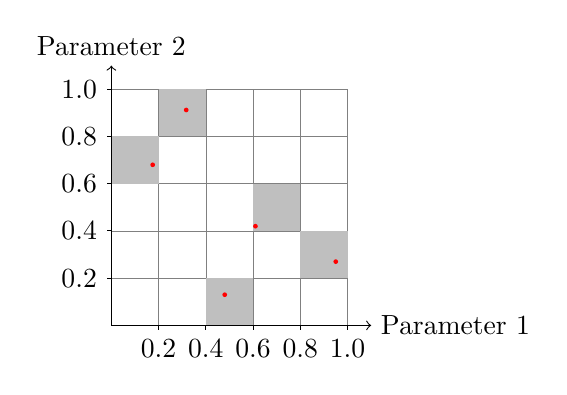
\begin{tikzpicture}[scale=3]

    % Define the grid
    \draw[step=0.2,gray,very thin] (0,0) grid (1,1);
    
    % Shade specific squares
    \fill[gray!50] (0.0,0.6) rectangle (0.2,0.8);
    \fill[gray!50] (0.2,0.8) rectangle (0.4,1.0);
    \fill[gray!50] (0.4,0.0) rectangle (0.6,0.2);
    \fill[gray!50] (0.6,0.4) rectangle (0.8,0.6);
    \fill[gray!50] (0.8,0.2) rectangle (1.0,0.4);
    
    % Draw red points
    \fill[red] (0.175,0.68) circle (0.01);  % Point in the first square
    \fill[red] (0.317,0.912) circle (0.01);  % Point in the second square
    \fill[red] (0.48,0.13) circle (0.01);  % Point in the third square
    \fill[red] (0.61,0.42) circle (0.01);  % Point in the fourth square
    \fill[red] (0.95,0.27) circle (0.01);  % Point in the fifth square
    
    % Draw the axes
    \draw[->] (0,0) -- (1.1,0) node[right] {Parameter 1};
    \draw[->] (0,0) -- (0,1.1) node[above] {Parameter 2};
    
    % Add ticks and labels
    \foreach \x in {0.2,0.4,0.6,0.8,1.0} {
      \draw (\x,0) -- (\x,-0.02) node[below] {\x};
      \draw (0,\x) -- (-0.02,\x) node[left] {\x};
    }
    
\end{tikzpicture}
    \caption{\acrshort{lhs} illustration}
    \label{fig:lhs}
\end{figure}

For the sampling experiment, \acrshort{lhs} was used with the same budget as other, i.e. 50 evaluations. Whole experiments took 36 hours. The aims of this experiments is dual: first, make a lower bound reference for others experiments, and second, explore the search space and the score behavior. To use as a lower bound, \acrshort{lhs} achieve scores of 37.6\% for MMLU, and 47.9\% for Hellaswag. Theses score are inside table \ref{tab:bounds}.

\begin{figure}
    \centering
    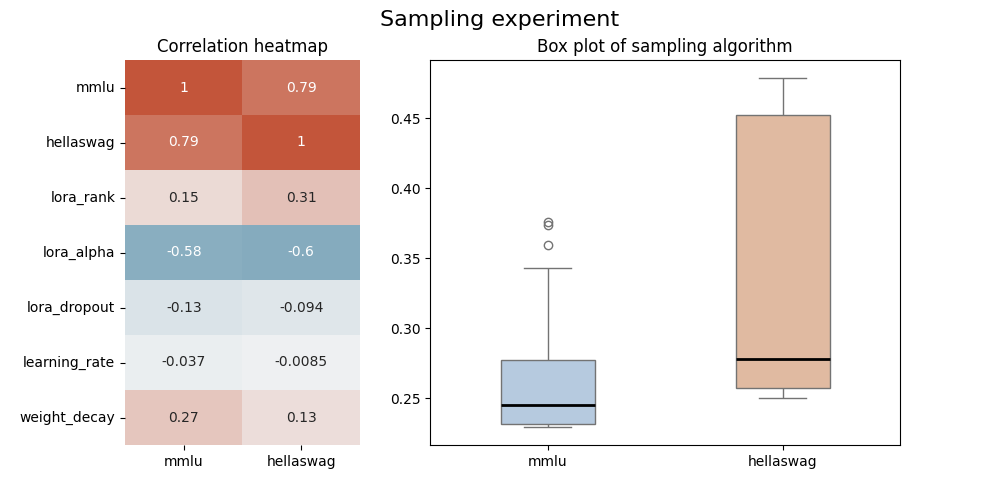
\includegraphics[width=0.6\linewidth]{assets/img/chap_4/experiments/plots/sampling/lhs.png}
    \caption{results of \acrlong{lhs} experiment}
    \label{fig:lhs_exp}
\end{figure}

The correlation between MMLU and Hellswag tend to confirm the relevance of their choice as a pair for validation and testing dataset. It's sufficiently high to guess that most of \textit{good} model for one will be good for the other one, but it's still less than one, making over-fitting visible if present.

For variables, it look like LoRA alpha, the scaling parameter of LoRA, is the most influent on the score, be it Hellaswag or MMLU. Next to it, LoRA Rank and weight decay are the most influent, with a difference in ranking on the metrics. With this first exploration, it look like Dropout and Learning rate are not very effectful for this problem, be it the choice of their range or the implementation. 

On the distribution of the score values, it's interesting to note that Hellaswag has a broader range of score, making it useful for efficiently discriminating solutions.  With a broader thinking, the sampling experiment confirm the relevance to apply \acrshort{hpo} algorithms to the described problem. If scores were independent from variables, or all scores were the same, \acrshort{hpo} would be useless. 

%%%%%%%%%%%%%%%%%%%% BO Experiment %%%%%%%%%%%%%%%%%%%%%%%%%%
\subsection{\acrshort{bogp} experiment}
\label{sec:bo_exp}

Figure \ref{fig:bo_res} depicts the performance of \acrfull{bogp} over 50 iterations, measured in terms of the \Gls{hs} accuracy. This visualization highlights the evolution of the optimization process as it transitions from sampling to the exploitation, and ultimately converges towards high-performing solutions.


\begin{figure}[h!]
    \centering
    \begin{subfigure}[b]{.50\textwidth}
      \centering
      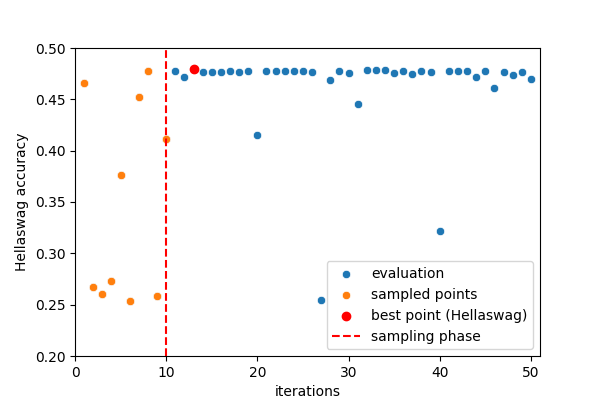
\includegraphics[width = \textwidth]{assets/img/chap_4/experiments/plots/bo/score_evolution.png}
      \caption{Score over time}
      \label{fig:bo_score_time}
    \end{subfigure}%
    \begin{subfigure}[b]{.40\textwidth}
      \centering
      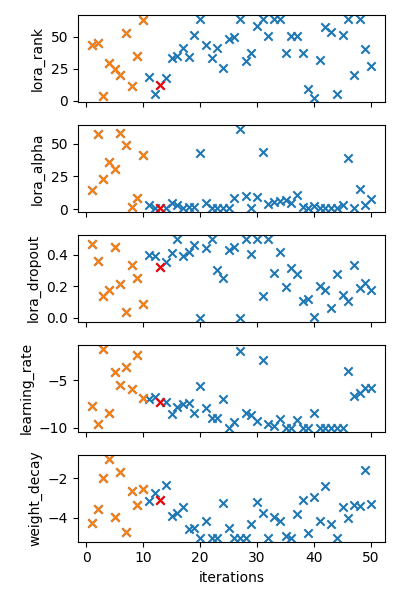
\includegraphics[width = 0.6\textwidth]{assets/img/chap_4/experiments/plots/bo/variables_evolution.png}
      \caption{Variable over time}
      \label{fig:bo_var_time}
    \end{subfigure}
    \caption{Experiment using \acrshort{bo} algorithm}
    \label{fig:bo_res}
\end{figure}

During the sampling phase, as shown by figure \ref{fig:bo_score_time}, evaluated solutions have the same diversity of solutions than the full sampling experiment, allowing to efficiently extract knowledge from the search space. The algorithm achieve a stable convergence to mostly high-performing solution.

If we briefly look at figure \ref{fig:bo_var_time}, it's interesting to look at the diversity of configuration to obtain high-performance, and the trend of the algorithms for each variables. For example, for LoRA alpha, or learning rate, we can observe a clear trend toward the lower bound of the optimization range. 

To summarize, this experiment demonstrate the effectiveness of Bayesian Optimization in efficiently exploiting the knowledge of the search space obtained in the sampling phase. The optimization process still explore area with high uncertainty, giving few low-performing solution.


%%%%%%%%%%%%%%%%%%%% SOO Experiment %%%%%%%%%%%%%%%%%%%%%%%%%%
\subsection{\acrshort{soo} experiment}
\label{sec:soo_exp}
On this experiment, we observe in Figure \ref{fig:soo_res} the behavior of \acrshort{soo} as it optimizes the given objective function. The figure illustrates how the algorithm navigates the search space, iteratively improving the solution by adjusting the hyperparameters. By examining the trends in performance metrics and variables evolution, we aim to analyze the convergence behavior, stability, and overall effectiveness of \acrshort{soo} in this setting.

\begin{figure}[h!]
    \centering
    \begin{subfigure}[b]{.5\textwidth}
      \centering
      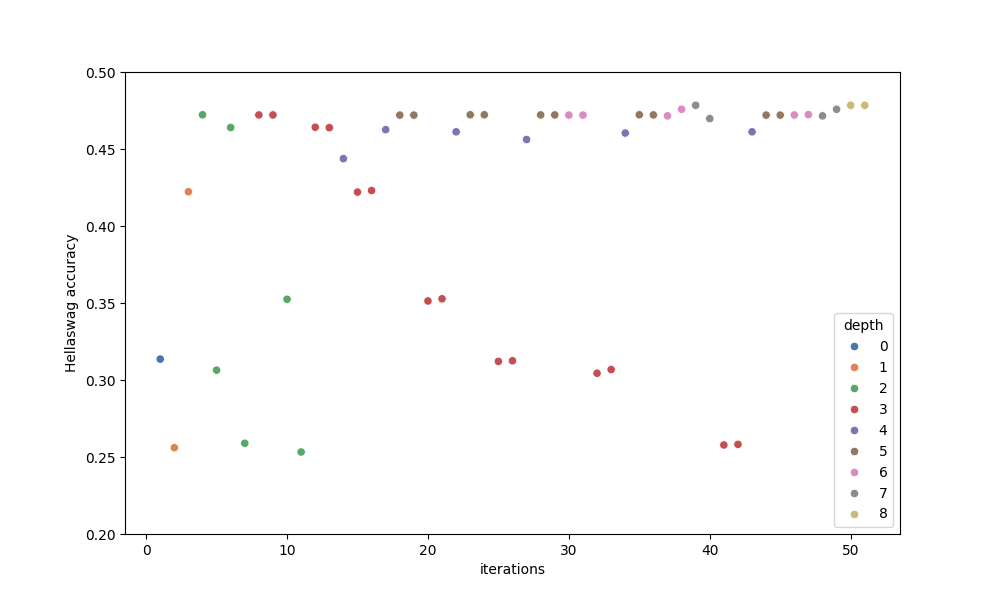
\includegraphics[width = \textwidth]{assets/img/chap_4/experiments/plots/soo/score_evolution.png}
      \caption{Score over time}
      \label{fig:soo_score_time}
    \end{subfigure}%
    \begin{subfigure}[b]{.4\textwidth}
      \centering
      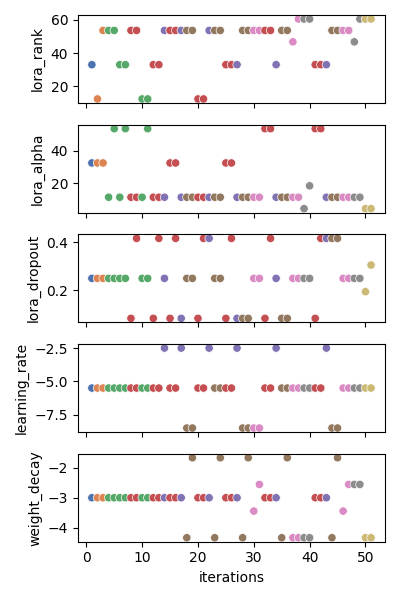
\includegraphics[width = 0.5\textwidth]{assets/img/chap_4/experiments/plots/soo/variables_evolution.png}
      \caption{Variable values over time}
      \label{fig:soo_var_time}
    \end{subfigure}
    \caption{Experiment using \acrshort{soo} algorithm}
    \label{fig:soo_res}
\end{figure}


Figure \ref{fig:soo_score_time} depicts the accuracy of the \gls{hs} dataset as a function of iterations, with marker colors representing different depth configurations. The observed trend suggests that most configurations achieve accuracies arround 0.46 throughout the optimization process. Several configurations converge toward the higher end of this range, indicating potential stability and effectiveness in learning as iterations progress. 

It is evident that higher-depth configurations tend to cluster around higher accuracy values, while lower depths display more scattered behavior across the accuracy spectrum. In specific, depth 2, with a section on lora alpha seems to greatly affect the performance on the accuracy. On figure \ref{fig:soo_var_time}, it's clear on the limitation of constrained-budget \acrshort{soo} without local exploitation at the end of the algorithms : Only a few number of values by variables are explored : around 5 by variables, making it equivalent to exploration of a search space of $6^5=7,776$ discrete solutions.

To summarize, \acrshort{soo} achieve a maximum performance closed to the precedent algorithm, but explore a restricted number of configuration, and lose time by evaluating unpromising solutions.

%%%%%%%%%%%%%%%%%%%% BaMSOO Experiment %%%%%%%%%%%%%%%%%%%%%%%%%%
\subsection{\acrshort{bamsoo} experiment}
\label{sec:bamsoo_exp}
The last experiment of this work is using \acrshort{bamsoo}, with $\eta = 1$ in equation \ref{eq:ucb}, to reduce the confidence interval and promote approximation, to avoid the evaluation of unpromising points. To look after it, figure \ref{fig:bamsoo_score_time} discriminate evaluated and approximated points, and might be compared with \ref{fig:soo_score_time} to look after approximated points.



\begin{figure}[h]
    \centering
    \begin{subfigure}[b]{.5\textwidth}
      \centering
      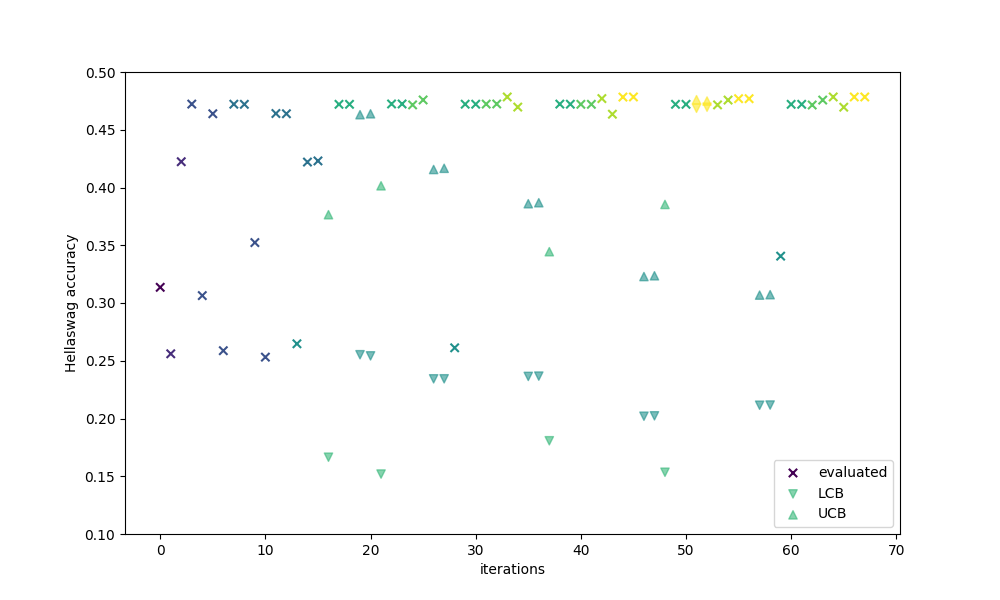
\includegraphics[width = 0.9\textwidth]{assets/img/chap_4/experiments/plots/bamsoo/score_evolution.png} 
      \caption{Score over time}
      \label{fig:bamsoo_score_time}
    \end{subfigure}%
    \begin{subfigure}[b]{.4\textwidth}
      \centering
      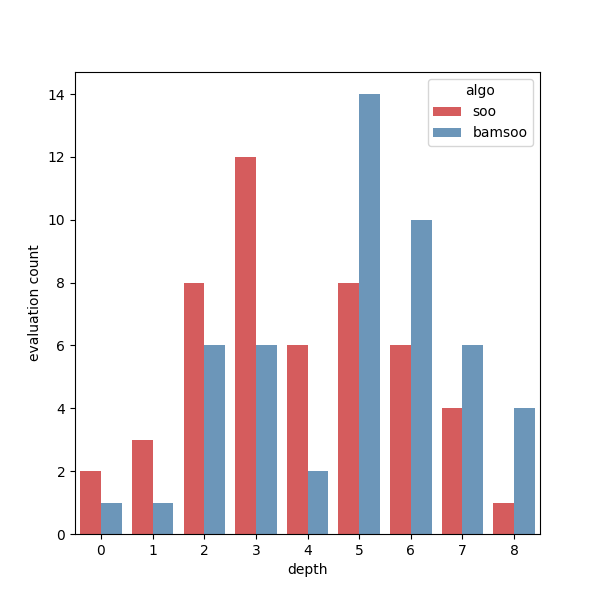
\includegraphics[width = 0.7\textwidth]{assets/img/chap_4/experiments/plots/bamsoo/depth_compar.png} 
      \caption{Depth exploration }
      \label{fig:bamsoo_soo_depth}
    \end{subfigure}
    \caption{Experiment using \acrshort{bamsoo} algorithm}
    \label{fig:bamsoo_res}
\end{figure}

When compared to figure \ref{fig:soo_score_time}, the pair of evaluations for depth 2, with low-performing solutions seems to have mostly been approximated. On the whole experiment, 16 points were approximated, to efficiently search further than \acrshort{soo}. Figure \ref{fig:bamsoo_soo_depth} compare the budget allowed on each depth, and highlight the focus of \acrshort{bamsoo} for lower depth exploration.
To summarize, \acrshort{bamsoo} achieve to speed up \acrshort{soo}, but is still slow in comparison with \acrshort{bo} at first glance. Moreover, \acrshort{bamsoo} succeed to prevent most of low-performing evaluation of \acrshort{soo}.


%%%%%%%%%%%%%%%%%%%%%%%%%% Analysis %%%%%%%%%%%%%%%%%%%%%%%%%%
\subsection{Comparison and analysis}
\label{sec:exp_analysis}
To conclude this section, it's crucial to directly compare algorithms, especially their performance, with validation and testing dataset. To look at absolute performance, and not only relative between algorithms, lower and upper bounds will be used. 

\begin{table}[h!]
    \centering
    \begin{tabular}{|c||c|c||c|c|c|}
    \hline
       Datasets  & Lower (LHS) & Upper (model card) & BO-GP & SOO & BaMSOO \\
    \hline
       Hellaswag (validation)  & 47.90 & 41.5 & 47.91 & 47.84 & 47.84\\
       MMLU (testing) & 37.61 & 49.3 & 38.11 & 37.42 & 37.50 \\
    \hline
    \end{tabular}
    \caption{Bounds on accuracy for validation and testing dataset}
    \label{tab:bounds}
\end{table}
In face of such experiments, it's interesting to look at bounds of the metric, to compare the results. The lower bounds is the results of the experiment using solely \acrshort{lhs} to pick solutions, with the same number of evaluation than algorithms. \acrshort{lhs} being intrinsically parallel, if evaluated algorithms don't achieve better performance than a solely exploring one, their benefit isn't relevant. 

For the higher bound, I will look at the higher value in the model card\footnote{\url{https://huggingface.co/meta-llama/Llama-3.2-1B}} of the model, achieved using advanced fine-tuning methods like Supervised Fine-Tuning (SFT), Rejection Sampling (RS), and Direct Preference Optimization (DPO). Values are inside table \ref{tab:bounds}.

\begin{figure}[h]
    \centering
    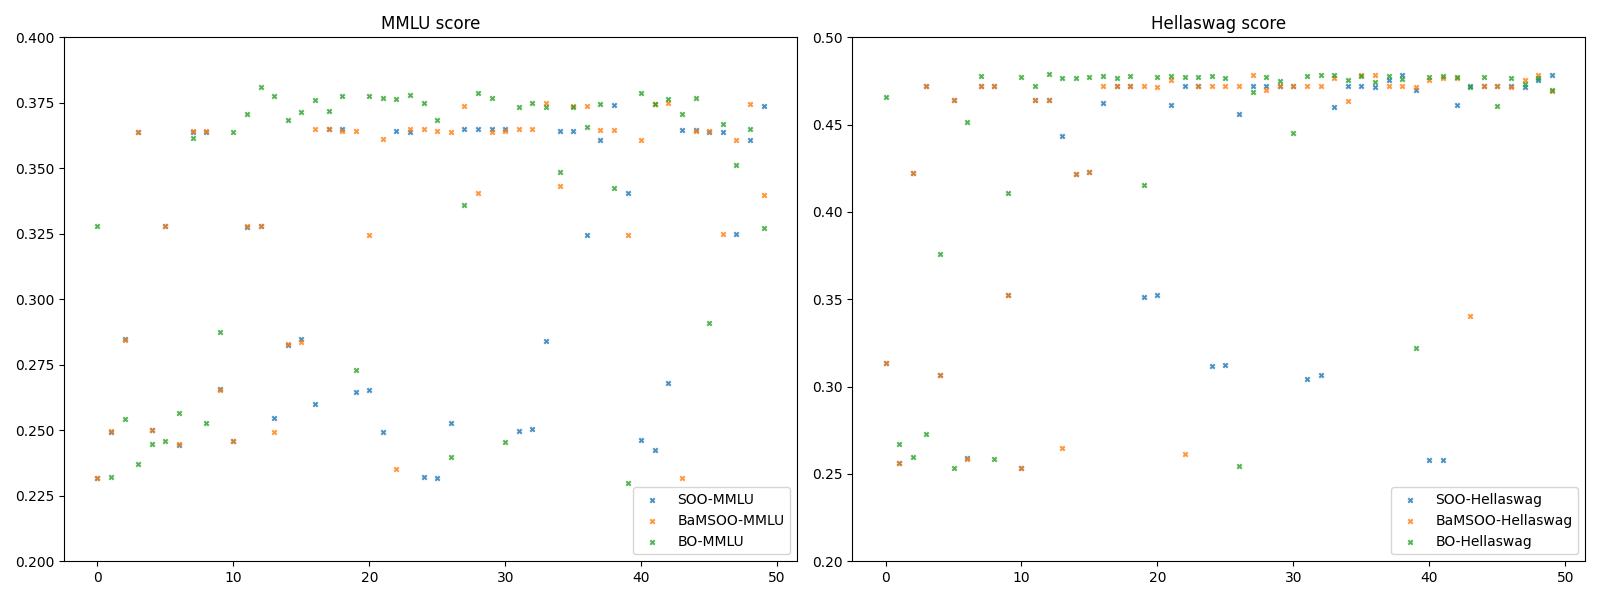
\includegraphics[width=0.8\textwidth]{assets/img/chap_4/experiments/plots/global/comparison.png}
    \caption{Comparison between 3 algorithms on 2 metrics}
    \label{fig:global_compare}
\end{figure}


At first, what's interesting is to look at testing and upper bounds results. Since the upper bound is mostly fine-tuned with aimed for MMLU results, the \Gls{hs} upper bounds isn't really relevant. Considering this, the analysis of this part will mostly be done with MMLU. The best results with MMLU is \acrfull{bo}, being 23\% from the upper bound.




With figure \ref{fig:global_compare}, it's clear than \acrshort{bo} algorithm is a step more performing than others algorithms for this problem, especially with the low number of low-performing solutions evaluated. Apart from this part, the whole results may suggest that the objective function, or the search space could be different, to have an higher range of results for comparison. 


%%%%%%%%%%%%%%%%%%%%%%%%%% Article Publication %%%%%%%%%%%%%%%%%%%%%%%%%%
\section{Article Publication}
\label{sec:article}

After few weeks of my internship, when we were able to define cleary a subject and estimate the possible contribution, with my supervisor we decided to aim to write an article from what I worked on. This aims push me to refine clearly what would be my contribution, since a published paper should aim for this. 

Under my supervisor guidance, what we aimed for was a conference article, for the International Conference on Optimization \& Learning (OLA2025). With this, a long paper should be published in \textit{Springer} indexed proceedings. At the time of writing and sending this report, the paper is under review, and the outcome is awaited. The current version can be found on github\footnote{\url{https://github.com/Kiwy3/ST30-deliverables/blob/master/OLA_Article/OLA.pdf}}

After a section on the contribution, I will adress in section \ref{sec:redaction} the redaction of the article, as it was also a crucial part of my internship.

%%%%%%%%%%%%%%%%%%%%%%%%%% Contribution %%%%%%%%%%%%%%%%%%%%%%%%%%
\subsection{The contribution}
\label{sec:contribution}
The first contribution of this work is direct and practical: the provision of usable \acrshort{hpo} algorithms and experiments specifically tailored for \acrshort{llm} \gls{fine_tuning}. The popularization of \acrshort{llm}s is a relatively recent development, and while these models are increasingly adopted by companies and end-users, the process of \gls{fine_tuning} remains somewhat inaccessible due to knowledge barriers and the lack of practical resources. By providing detailed experiments and insights into \acrshort{hpo} algorithms, this work aims to lower these barriers, enabling users to better understand and utilize \gls{fine_tuning} techniques. Furthermore, this contribution supports the selection of \glspl{hyperparameter}—a crucial step in achieving optimal performance without excessive trial and error.

The second contribution lies in addressing the challenge of optimizing expensive functions. The development and training of \acrshort{ann}s are computationally intensive processes, underscoring the importance of efficient optimization methods. This has driven significant interest in \acrshort{bo} algorithms, originally developed for scenarios such as mechanical and aeronautical engineering, where simulations can take hours to run. However, other domains with similarly expensive functions stand to benefit from advancements in this area. Through this work, a comparative analysis was conducted between two approaches for optimization in settings with limited evaluations, providing valuable insights for both researchers and practitioners.

Finally, this work contributes to the scalability of \acrshort{bo} algorithms. Given that this internship is part of an exascale computing project, the broader goal is to develop scalable and efficient algorithms capable of handling a wide variety of use cases. While the immediate focus has been on \acrshort{llm} \gls{fine_tuning}, the findings and methodologies have implications that extend to other computationally intensive tasks. By addressing scalability, this work lays the groundwork for future innovations in optimization methods that can leverage the full potential of high-performance computing infrastructure.


%%%%%%%%%%%%%%%%%%%%%%%%%% Redaction %%%%%%%%%%%%%%%%%%%%%%%%%%
\subsection{Redaction}
\label{sec:redaction}

The redaction was as interesting as it was frustating sometimes. To start, I looked at many articles structures, and talked with my supervisor to define the global contents of the article. With this first step, I wrote as early as possible what I could write without having results, to be able to step back on my own work, and see the limitations of what I have written. 

The end of the paper was a little bit more rushed, because I did not have correct and useful results before 2 days before the submission deadline. The time and ressource for one experiments were so that I could not launch a lot of experiment to do sufficient tests. 

In a technical aspect, the redaction of the article, like the redaction on this report was useful to learn how to use \LaTeX{}, from making tables and load figures, to the production of figures using \textit{Tikz} library. 


%%%%%%%%%%%%%%%%%%%%%%%%%% Challenges %%%%%%%%%%%%%%%%%%%%%%%%%%
\section{Challenges}
\label{sec:challenge}

This section outlines the key challenges encountered during the internship and the strategies employed to address them. Undertaking a project situated at the intersection of multiple research domains presented unique difficulties, from defining and addressing a novel research problem to managing the technical complexities of implementation and resource constraints. Each of these challenges required a combination of critical thinking, adaptability, and collaboration to overcome. The following sections delve into these obstacles in detail, highlighting the learning process and the methods used to navigate the intricacies of both the theoretical and practical aspects of the work.



%%%%%%%%%%%%%%%%%%%%%%%%%% Complex field %%%%%%%%%%%%%%%%%%%%%%%%%%
\subsection{Adress a research problematic}
\label{sec:adress_research}
The first significant challenge I faced during the initial weeks of my internship was adapting to a completely new environment and working on a subject rooted in research—a domain I had not fully encountered before. While my academic courses had involved numerous projects of varying complexity and levels of research ambition, this internship marked the first time I was required to address a genuine research problem in its entirety. This shift introduced me to the complexities of the research process and the skills necessary to navigate it effectively.

One of the initial hurdles was managing the literature review. This involved handling numerous references, reading and analyzing complex academic articles, and extracting relevant information to identify a specific research problem. Estimating the right problematic to focus on proved particularly difficult at the outset, given the broad scope and technical depth of the subject. However, with the guidance of my supervisor, I was able to refine my understanding of the domain, define a clear and well-scoped research problem, and develop a structured approach to tackle it. This process laid the foundation for the rest of the project, ensuring that my efforts were focused and aligned with the goals of the internship.


%%%%%%%%%%%%%%%%%%%%%%%%%% Complex field %%%%%%%%%%%%%%%%%%%%%%%%%%
\subsection{Work in a complex research field}
\label{sec:complex_field}
The subject of my internship was as fascinating as it was complex, sitting at the intersection of several cutting-edge research fields. To approach this multidisciplinary challenge effectively, I began with a rapid yet thorough literature review of each relevant aspect. This step was essential to grasp the stakes of the subject and avoid wasting valuable time on unnecessary or redundant work. The fields I needed to familiarize myself with included \acrshort{llm}, encompassing \acrshort{ann}s and the specific nuances of \acrlong{peft}, as well as \acrlong{bo}, which required an understanding of probabilistic models and optimization rules. Additionally, I had to delve into \acrfull{hpc}, particularly the scalability of processes, which became increasingly relevant to my project’s objectives.

This endeavor was particularly challenging for me because my aim was to produce work comparable to that of well-established researchers or even research teams, despite having only a short internship period of six months to achieve it. Starting from scratch, I had to quickly acquire foundational knowledge and develop expertise in these domains. Balancing the demands of mastering multiple complex fields while striving to meet the high standards of professional research pushed me to adapt and learn at an accelerated pace. This experience, while demanding, was invaluable in helping me grow both academically and professionally.


%%%%%%%%%%%%%%%%%%%%%%%%%% Technical implementation %%%%%%%%%%%%%%%%%%%%%%%%%%
\subsection{Technical implementation}
\label{sec:tech_impl}

The first significant difficulty I encountered was related to the development process itself. I lacked a well-structured approach to code development, including strategies for writing clean, efficient, and modular code, as well as systematic methods for testing it. This absence of an established process initially slowed down my progress and required me to learn best practices as I advanced through the project.

Another major challenge was working with numerous libraries for implementing the black-box objective function. The codebase involved a complex network of libraries, classes, and functions, all deeply interconnected. It was initially overwhelming to understand how these components interacted and to adapt the existing code to fit my specific requirements. This was especially challenging because my use case—\acrlong{hpo}—was not a generic application of the libraries. As such, no pre-existing implementation was readily available to use \acrshort{hpo} as a black-box objective function, requiring significant effort to tailor the code.

Resource limitations also posed a considerable obstacle. At the beginning of the project, I had to rely on Grid'5000 as the primary computational resource. While g5k provided an essential platform for experimentation, its limitations in terms of scalability and availability required careful management of resources and computational tasks. Overcoming these challenges not only helped me refine my problem-solving skills but also provided valuable experience in navigating the practical constraints of real-world computational research.
